The basic idea of Darwin method was introduced in~ \cite{GMS09}. This idea will
be described in the following paragraph.

\subsection{Background}

The method combines two different approaches --- Interactive Multiobjective
Optimisation (IMO, see~TODO) and Evolutionary Multiobjective Optimization
(EMO, see~TODO).

In the IMO paradigm we want to elicit Decision Maker (DM) preferences by
involving her in the process. This is done by systematic dialog with the
DM. Questions are being asked and the DM provides answers. Based on these
answers preference information is extracted. Algorithm can then use this
knowledge to produce solution better fitted to the Decision Maker
preferences. The IMO framework is presented on
fig.~\ref{fig:interactive-process}.

\begin{figure} 
  \begin{center}
    \begin{tikzpicture}
      \matrix[row sep=10mm, column sep=10mm]{

        
        \node (gen)     [roundrect] {
          \begin{tabular}{c}
            1. Generate set\\
            of possible solutions
        \end{tabular}}; &

        \node (ask) [roundrect] {
          \begin{tabular}{c}
            2. Ask the DM \\
            to indicate `good' ones
        \end{tabular}}; \\

        \node (use) [roundrect] {
          \begin{tabular}{c}
            4. Improve solution set
        \end{tabular}}; &

        \node (store) [roundrect] {
          \begin{tabular}{c}
            3. Extract \\
            preference information
        \end{tabular}}; \\
      };
      \path (gen) edge[->] (ask);
      \path (ask) edge[->] (store);
      \path (store) edge[->] (use);
      \path (use) edge[->] (gen);
    \end{tikzpicture}
    \caption{Typical Interactive Multiobjective
      Optimisation process framework\label{fig:interactive-process}}
  \end{center} 
\end{figure} 

Rationale behind the interactive process is that the Decision Maker is
interested only in a small subset of preferred solutions or even in a single
most preferred one.

This process makes possible to gather preference information and then use this
information to construct better solutions. However this is just a framework,
details are left up to analyst. Especially one has to think how to extract and
store knowledge gathered on DM's answers and how to use this knowledge to
generate and provide solutions better fitted to Decision Maker's
preferences.

Human factor is another thing to consider. DM is a human being and thus her
behavior is constantly changing. The challenge here is to find what questions
should be asked, how often and how many intermediate solutions should be
presented to evaluate. 

Evolutionary Multiobjective Optimisation (EMO) provides a computational engine
for generating new, better solutions from existing ones. Better in sense of
objective function defined in the solution space. Most of the EMO methods are
approximating Pareto-optimal front by a set of solutions. So one solution is
better than the other if the former Pareto-dominates the latter. In case of
two equivalent ones another factors have to be taken into account (for example
crowding score in NSGA2 [ref]). This is the case because if no preference
information is given all Pareto-optimal solutions have to be considered
equivalent.

It seems natural to combine these two approaches described --- Interactive
Multiobjective Optimisation and Evolutionary Multiobjective
Optimisation. (TODO: maybe a note and a ref about combining these two
approaches). IMO is just a process framework but still needs an engine to
generate and improve solutions. EMO is such an engine. On the other hand for
EMO involving the Decision Maker in the procedure results in gathering
preference information. This information allows the procedure to focus on
specific region of Pareto-front --- the one most relevant to decision maker.

\begin{figure}
  \centering \includegraphics[width=1.2\textwidth]{img/pareto}
  \caption{Pareto-front and area preferred by the Decision Maker}
  \label{pareto}
\end{figure}

This is important because of the ``human factor''. If a number of solution
becomes huge DM can not effectively analyze it and find the one that fits best
her preferences, thus Pareto-optimality is not sufficiently
discriminative. However guiding the search to preferred regions of the
solution space allows the method to coverage faster to good solutions. It is
shown on fig.~\ref{pareto}.


\subsection{Uncertainty}

TODO


\subsection{The algorithm}

DARWIN can operate on a Multi-Objective Optimisation (MMO) problems defined as
follows:

\begin{equation}
[ f_1(x), f_2(x), \dots, f_k(x) ] \rightarrow  \max
\end{equation}
subject to:
\begin{equation}
\begin{array}{l}
g_1(x) \geq b_1 \\
g_2(x) \geq b_2 \\
\dots \\
g_m(x) \geq b_m
\end{array}
\end{equation}

Where:
\begin{description}
\item $x = [x_1, x_2, \dots, x_n]$ is a vector of decision variables, called a
  solution;
\item $f_1(x), f_2(x), \dots, f_k(x)$ are objective functions,
  $f: x \rightarrow \mathbb{R}$;
\item $g_1(x), g_2(x), \dots, g_m(x)$ are constraint functions,
  $f: x \rightarrow \mathbb{R}$;
\item $b_1, b_2, \dots, b_m$ are real-valued right hand sides of the
  constraints.
\end{description}

\begin{figure}
  \centering 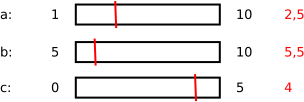
\includegraphics[width=0.5\textwidth]{img/scenario}
  \caption{Scenario --- set of intervals fixed on specific values}
  \label{scenario}
\end{figure}

It is possible to give some of the coefficients in objective functions or
constraints in form of intervals (thus modeling ignorance --- uncertainty
about real value of an coefficient). A vector of fixed values for each
interval is called \textit{scenario} of imprecision (see fig.~\ref{scenario}).

DARWIN is composed of two nested loops --- exterior and interior. The former
is a realisation of an interactive process and the latter is an EMO engine
dedicated to improve solutions based on the Decision Maker preferences. This
is illustrated on figure~\ref{fig:darwin-ext}.

\begin{figure} 
  \begin{center}
    \begin{tikzpicture}
      \matrix[row sep=10mm, column sep=10mm]{

        
        \node (gen)     [roundrect] {
          \begin{tabular}{c}
            (0) Generate:\\
            * solutions\\
            * scenarios
        \end{tabular}}; &

        \node (presentation) [greenrect] {
          \begin{tabular}{c}
            (1) Presentation \\
            of results
        \end{tabular}}; &

        \node (eval) [greenrect] {
          \begin{tabular}{c}
            (2) DM\\
            evaluation
        \end{tabular}}; \\

        \node (stop) [redrect] {
          \begin{tabular}{c}
            STOP
        \end{tabular}}; &

        \node (inner) [greenrect] {
          \begin{tabular}{c}
            (4) Evolutionary \\
            loop
        \end{tabular}}; &

        \node (rules) [greenrect] {
          \begin{tabular}{c}
            (3) Rules \\
            generation
        \end{tabular}}; \\
      };
      \path (gen) edge[->] (presentation);
      \path (presentation) edge[->] (eval);
      \path (eval) edge[->] (rules);
      \path (rules) edge[->] (inner);
      \path (inner) edge[->] (presentation);
      \path (presentation) edge[->] (stop);
    \end{tikzpicture}
    \caption{DARWIN states and transitions. Steps (1) - (4) are forming
      exterior loop and step (4) is the interior loop.\label{fig:darwin-ext}}
  \end{center} 
\end{figure}


The exterior loop is composed of the following steps.

\begin{algorithm}
\caption{DARWIN's exterior loop}\label{extloop}
  \begin{algorithmic}[1]
    \While{}
    \EndWhile{}
  \end{algorithmic}
\end{algorithm}

\begin{description}
  \item[Step 1.] Generate set of feasible solutions $X$ to the problem
  
\end{description}
